% Section content template for individual Educative lessons
% This file contains the actual content for a specific section
% Generated from Educative API section content

% Section: Activity Diagram for the Amazon Online Shopping System
% Section ID: 5911026583470080
% Section Slug: activity-diagram-for-the-amazon-online-shopping-system
% Generated: 2025-12-12T22:46:02.304863

Activity diagrams are a great way to visualize the flow of messages from one activity to another in the system. There can be different activity diagrams that we can create for our Amazon online shopping system. In this lesson, we will create activity diagrams for the following two activities:

\begin{itemize}
\item
\protect\phantomsection\label{tJjlB9a0P4DGp3YYVnVdK}
A customer is buying a product.
\item
\protect\phantomsection\label{Sp7IKa-4DI_BcL-QOwgNZ}
\textbf{Activity challenge:} The customer receives their order.
\end{itemize}

\subsection{A customer buying a product}\label{dsU47-_mvo_p-Ks4_OlYn}
\\
The following are the states and actions that will be involved in this activity diagram.

\subsubsection{States}\label{qHTw_o-s1d4h2NOwC-dt8}
\\
\textbf{Initial state:} The customer opens Amazon.
\\
\textbf{Final state:} The customer proceeds with checkout.

\subsubsection{Actions}\label{MBYKQdPw8SUzn0JM9bwk1}
\\
The customer opens the website. They search or browse the website, select a product, and buy it.

\begin{figure}[htbp]
 \centering
 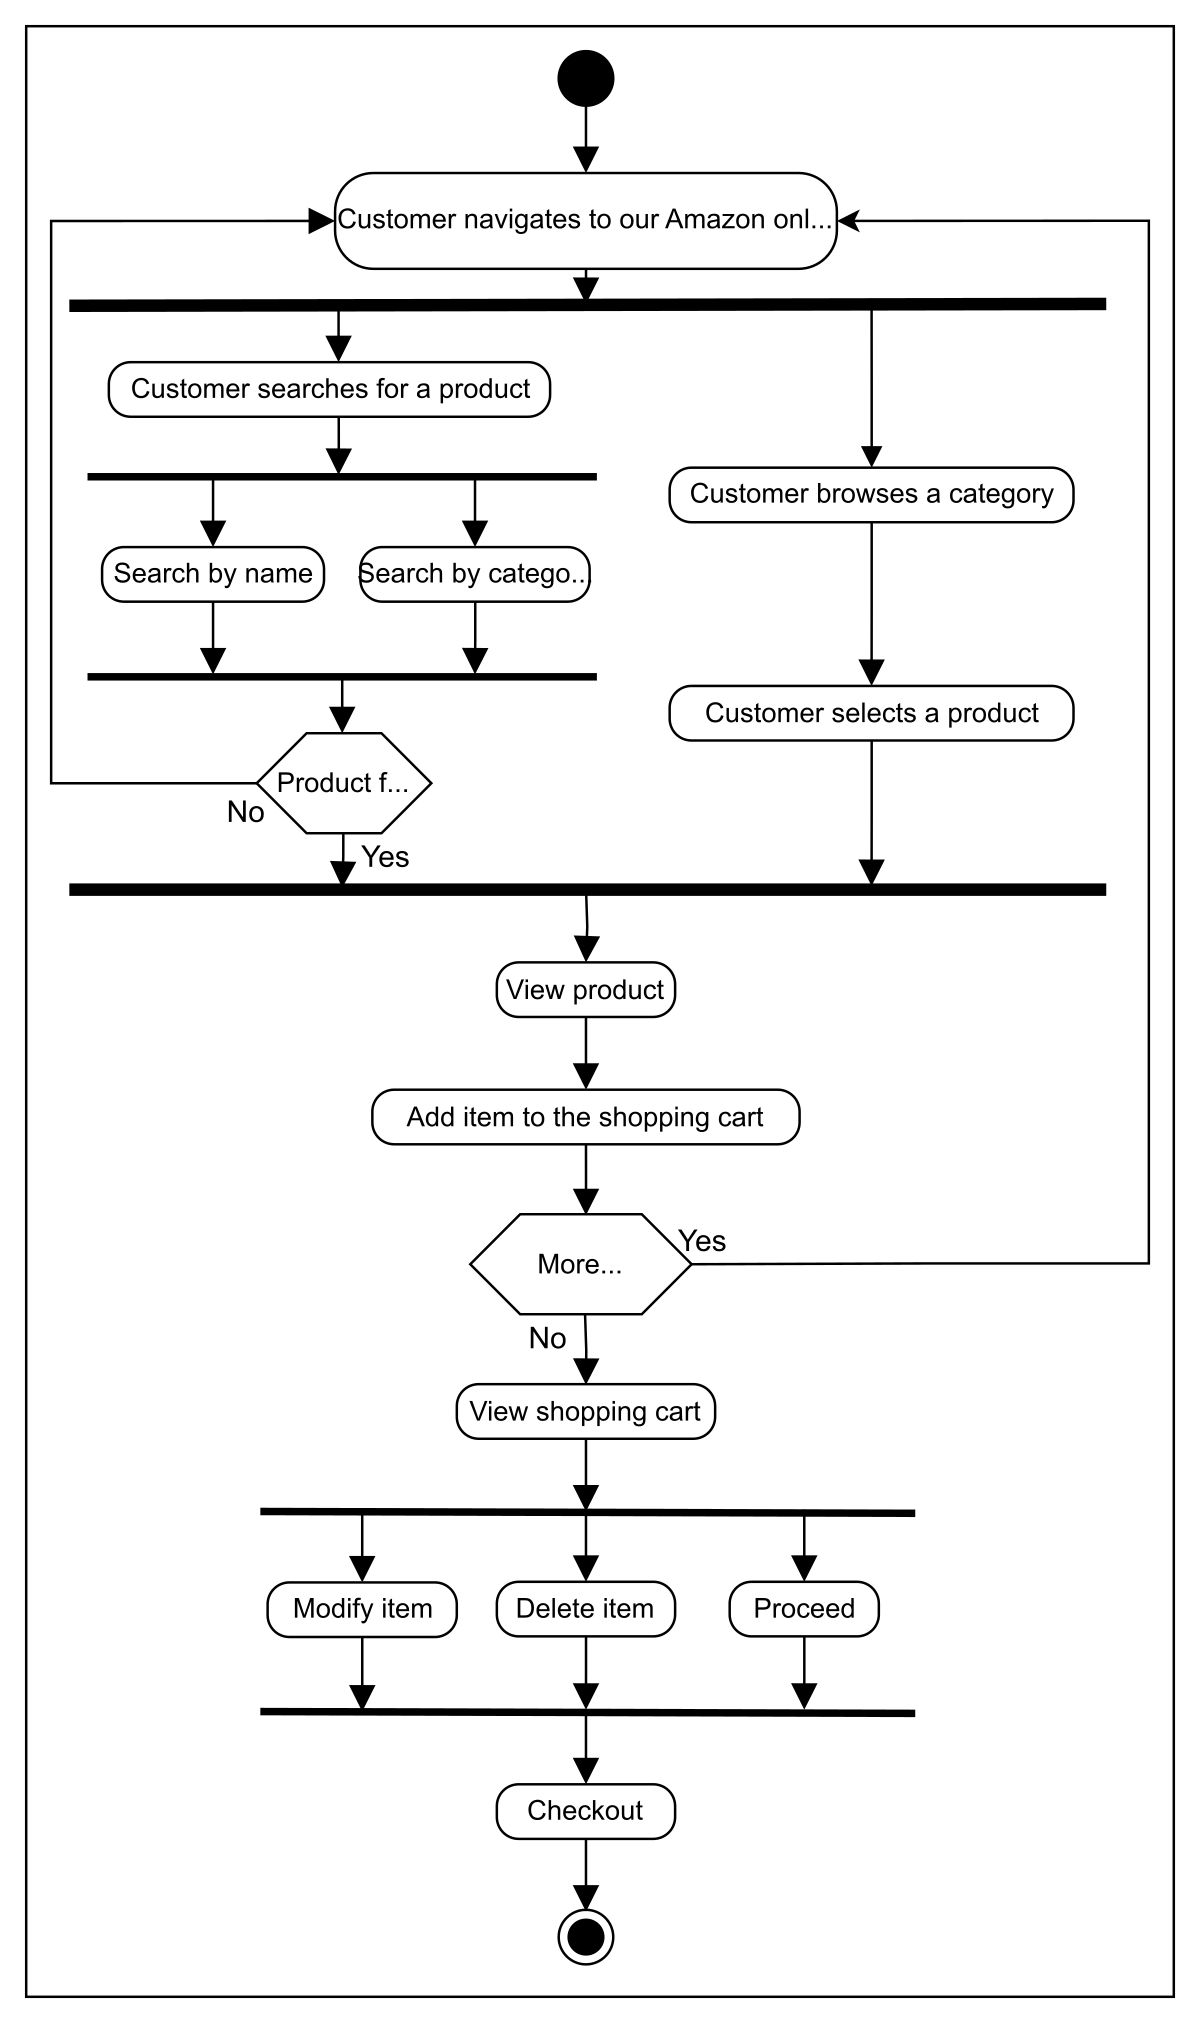
\includegraphics[width=0.5\textwidth]{Images/chapter_19/section_5911026583470080/6203553616887808.png}
 \caption{The activity diagram for a customer buying a product}
\end{figure}

\subsection{Activity challenge: Customer order checkout and payment process}\label{qQ8UiLDWEEf6Cnibbq9TJ-2}
\\
You'll help us create an activity diagram for a customer order checkout and payment process. In this activity, the customer checks out and selects a payment method---cash on delivery or credit card---before checkout.
\\
A skeleton of the activity diagram is provided below.

\begin{figure}[htbp]
 \centering
 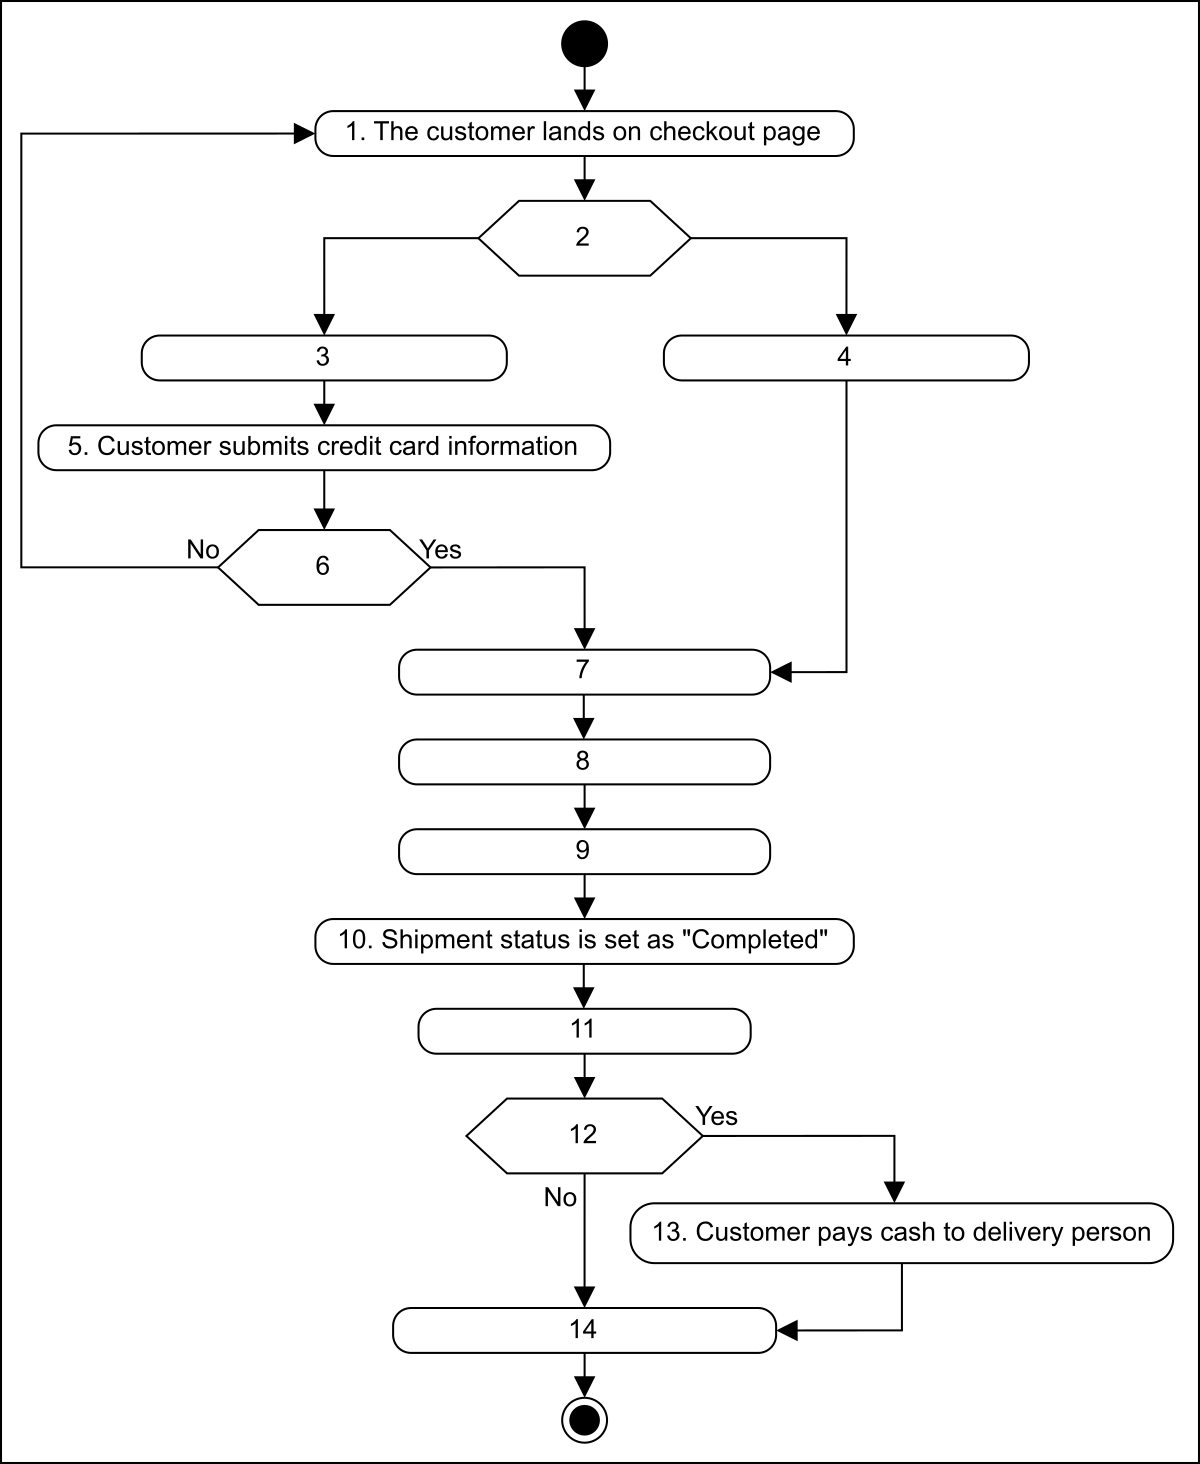
\includegraphics[width=0.5\textwidth]{Images/chapter_19/section_5911026583470080/5560415993200640.png}
 \caption{The activity diagram for a customer receiving their order}
\end{figure}

Notice that the actions in the diagram above are numbered from 1 to 14. The slots below represent the activities, and the arrows represent the flow from one activity to another.
\\
Can you rearrange the slots below in the correct order they should appear in the activity diagram above?
\begin{quote}
\textbf{Note:} If you're stuck, click the ``Show Solution'' button.
\end{quote}


Alternatively, you can click the ``Show complete diagram'' button below to see the complete activity diagram.

We've looked at some of the activity diagrams of our Amazon online shopping system. In the next lesson, we'll present the code for our designed classes in some of the most popular languages.

% End of section content